\documentclass[11pt]{article}
\usepackage[a4paper, margin=1in]{geometry}
\usepackage{amsmath}
\usepackage{amssymb}
\usepackage{amsthm}
\usepackage{booktabs}
\usepackage{graphicx}
\usepackage{xcolor}
\usepackage{listings}
\usepackage{hyperref}
\hypersetup{colorlinks=true, urlcolor=blue!55!black, linkcolor=blue!55!black,
            citecolor=blue!55!black}
\lstdefinestyle{py}{language=Python, basicstyle=\ttfamily\scriptsize,
  keywordstyle=\color{blue!60!black}, commentstyle=\color{green!45!black},
  stringstyle=\color{red!55!black}, numbers=left, numberstyle=\tiny\color{gray},
  numbersep=6pt, breaklines=true, showstringspaces=false, columns=fullflexible,
  keepspaces=true, frame=single, framerule=0.3pt, rulecolor=\color{gray!40},
  tabsize=4, upquote=true, xleftmargin=1.5em}
\newtheorem{definition}{Definition}
\newtheorem{proposition}{Proposition}

\title{\textbf{Order Flow Imbalance and Price Impact\\ in a Limit Order Book}\\[3pt]
\large Multi-Level and Integrated OFI on Real NASDAQ Data,\\
with Contemporaneous and Out-of-Sample Analysis}
\author{Godfred Antwi Koduah\\
\small Ph.D.\ Student, Financial Mathematics, Florida State University}
\date{}

\begin{document}
\maketitle

\begin{abstract}
\noindent Order flow imbalance (OFI) --- the net pressure of buy versus sell
activity in a limit order book --- is among the most robust explanators of
short-horizon price movement. Using real level-10 NASDAQ order-book data for AAPL
(LOBSTER sample, 21 June 2012; 400{,}391 events over 6.5 trading hours), I
reconstruct OFI from first principles at every book level, and study its
relationship to price both contemporaneously and predictively. A single
best-level OFI regressor explains $30\%$ of contemporaneous one-second mid-price
changes; using all ten levels raises this to $50\%$, and a single
PCA-\emph{integrated} OFI factor recovers nearly all of that gain ($48.5\%$),
showing that the deep book carries substantial price information beyond the top of
book. The contemporaneous fit strengthens monotonically with the aggregation
horizon, reaching $R^2=0.74$ (multi-level) at thirty seconds, and the estimated
price-impact coefficient is strongly significant under Newey--West inference
(HAC $t\approx 11$). In sharp contrast, lagged OFI has almost no out-of-sample
predictive power ($R^2\approx 0.007$ at one second) --- the expected signature of
an efficient market in which OFI moves price concurrently rather than forecasting
it. The study is fully reproducible from the public sample and the code included
here.
\end{abstract}

\tableofcontents
\bigskip

\section*{Key findings}
\addcontentsline{toc}{section}{Key findings}
\begin{itemize}
\item Best-level OFI explains $30.1\%$ of contemporaneous 1-second mid-price
changes on real AAPL data; all ten levels together explain $50.5\%$.
\item A single PCA-integrated OFI factor captures $48.5\%$ --- almost the entire
multi-level gain --- so the extra information in the deep book is largely
one-dimensional.
\item Contemporaneous explanatory power rises with horizon: $R^2$ for multi-level
OFI is $0.51$ (1s), $0.64$ (5s), $0.67$ (10s), $0.74$ (30s).
\item The price-impact coefficient is positive and strongly significant under
Newey--West (HAC) standard errors ($t\approx 11$).
\item Lagged OFI is \emph{not} predictive out of sample ($R^2\approx 0.007$,
shrinking with horizon), consistent with near-efficiency: OFI accompanies price
formation, it does not forecast it.
\item The impact is approximately \emph{linear} in OFI (binned $R^2=0.94$) and
\emph{permanent} (about $131\%$ of the immediate move persists after 20s), and the
impact coefficient varies roughly threefold through the trading day.
\end{itemize}
\bigskip

\section{Introduction}
When a trade or quote update arrives, it does not move price at random: it moves
price in the direction of the net order flow it represents. \emph{Order flow
imbalance} (OFI) quantifies that net pressure from changes in the quoted sizes and
prices on each side of the book, and a large microstructure literature establishes
it as the dominant driver of short-horizon price change \cite{cks2014}. This
report studies OFI from first principles on real data, with three questions in
view. First, how much of contemporaneous price movement does OFI explain, and does
the \emph{deep} book add to what the top of book already tells us? Second, is the
relationship stable across time scales and statistically robust once serial
correlation is accounted for? Third --- the question that separates a describable
regularity from a tradeable one --- does OFI \emph{predict} future returns out of
sample, or only move with price concurrently?

\paragraph{Scope.} This is a single-asset, single-day study on the public LOBSTER
AAPL sample. That is enough to establish the OFI--price-impact relationship
rigorously and to separate contemporaneous explanation from out-of-sample
prediction. The multi-asset \emph{cross}-impact extension of
\cite{ccz2023} --- where one asset's order flow moves another's price --- requires
synchronized multi-ticker data and is left as clearly-scoped future work.

\section{Data}
The LOBSTER sample reconstructs the NASDAQ limit order book for AAPL on
21 June 2012 to ten levels per side, from the official ITCH message stream
\cite{lobster}. Two aligned files are used: a \emph{message} file (one row per
event: timestamp, type, order id, size, price, direction) and an \emph{order-book}
file (one row per event giving, for each of ten levels, the ask price, ask size,
bid price, and bid size). After the opening, the sample contains $400{,}391$
events spanning $34{,}200$--$57{,}600$ seconds (09:30--16:00), i.e.\ $6.5$ hours.
The mid-price ranges over \$577.48--\$588.18 and the mean quoted spread is
\$0.154. Row $i$ of the order-book file is the state of the book immediately after
message $i$, so the two files together give a complete, event-by-event history of
the top ten levels.

\section{Method}

\subsection{Order flow imbalance at a single level}
Let the best bid be $(P^b_n, q^b_n)$ and best ask $(P^a_n, q^a_n)$ after event
$n$. Following Cont, Kukanov and Stoikov \cite{cks2014}, the bid-side order-flow
contribution of event $n$ is
\begin{equation}
\Delta W^b_n =
\begin{cases}
q^b_n, & P^b_n > P^b_{n-1} \quad (\text{bid improves}),\\
q^b_n - q^b_{n-1}, & P^b_n = P^b_{n-1} \quad (\text{same level}),\\
-\,q^b_{n-1}, & P^b_n < P^b_{n-1} \quad (\text{bid falls}),
\end{cases}
\end{equation}
and symmetrically for the ask side,
\begin{equation}
\Delta W^a_n =
\begin{cases}
q^a_n, & P^a_n < P^a_{n-1} \quad (\text{ask improves, i.e.\ falls}),\\
q^a_n - q^a_{n-1}, & P^a_n = P^a_{n-1},\\
-\,q^a_{n-1}, & P^a_n > P^a_{n-1}.
\end{cases}
\end{equation}
The per-event order flow imbalance is $e_n = \Delta W^b_n - \Delta W^a_n$, and the
OFI over a time bucket $[\tau, \tau+h)$ is the sum of its events,
\begin{equation}
\mathrm{OFI}_\tau = \sum_{n:\ t_n \in [\tau,\tau+h)} e_n .
\end{equation}
The sign convention is such that net buying pressure (bid built up, ask consumed)
gives $\mathrm{OFI} > 0$, which should push the price up.

\subsection{Multi-level and integrated OFI}
The same construction applies at each book level $m = 1,\dots,10$, using that
level's price and size, producing $\mathrm{OFI}^{(m)}_\tau$. Deeper levels carry
information that the top of book does not --- liquidity replenishment and
withdrawal below the touch presage where price can go. Rather than treat the ten
series as ten free regressors (which risks collinearity), I follow the integrated
construction of \cite{ccz2023}: standardize each level's OFI, and take the first
principal component of their covariance matrix,
\begin{equation}
\mathrm{OFI}^{\mathrm{int}}_\tau = \sum_{m=1}^{10} w_m\, \widetilde{\mathrm{OFI}}^{(m)}_\tau,
\qquad w = \text{first eigenvector of } \operatorname{Cov}\big(\widetilde{\mathrm{OFI}}\big),
\end{equation}
where $\widetilde{\cdot}$ denotes standardization. This yields a single, robust
depth-weighted factor.

\subsection{Price impact and inference}
The contemporaneous price-impact model regresses the mid-price change over a
bucket (in cents) on the bucket's OFI,
\begin{equation}
\Delta \mathrm{mid}_\tau = \alpha + \lambda\, \mathrm{OFI}_\tau + \varepsilon_\tau,
\label{eq:impact}
\end{equation}
with $\lambda$ the price-impact coefficient. Because bucketed microstructure
series are serially correlated and heteroskedastic, ordinary OLS standard errors
understate uncertainty; I report Newey--West (HAC) standard errors with Bartlett
weights,
\begin{equation}
\widehat{\operatorname{Var}}(\hat\beta) = (X^\top X)^{-1}
\Big(\hat\Omega_0 + \sum_{l=1}^{L}\big(1-\tfrac{l}{L+1}\big)(\hat\Omega_l + \hat\Omega_l^\top)\Big)
(X^\top X)^{-1},
\end{equation}
with $\hat\Omega_l$ the lag-$l$ autocovariance of the score $x_i \hat\varepsilon_i$
and $L=10$.

\subsection{Out-of-sample predictive test}
Contemporaneous explanation does not imply forecasting power. To test prediction
honestly I regress the \emph{next} bucket's return on the current OFI,
$\Delta \mathrm{mid}_{\tau+1} = \alpha + \beta\,\mathrm{OFI}_\tau + \varepsilon$,
estimate $(\alpha,\beta)$ on the first half of the trading day, and evaluate
$R^2$ on the held-out second half. The split is chronological, so no future
information enters the fit.

\section{Results}

\subsection{Contemporaneous impact and the value of depth}
At one-second buckets ($21{,}029$ observations), best-level OFI alone explains
$R^2 = 0.301$ of mid-price changes (Figure~\ref{fig:impact}), with a positive,
strongly significant impact coefficient ($\lambda = 4.08\times10^{-3}$ cents per
unit, Newey--West $t = 11.0$). Using all ten levels raises $R^2$ to $0.505$, and
the single integrated factor recovers $0.485$ --- almost the entire gain from one
extra degree of freedom (Table~\ref{tab:main}). Every level carries price
information individually (Figure~\ref{fig:levels}; per-level $R^2$ ranges
$0.22$--$0.30$), and the first principal component accounts for $53.7\%$ of the
level-OFI covariance, so the deep-book signal is largely one-dimensional --- which
is exactly why a single integrated factor works so well.

\begin{table}[h]
\centering
\begin{tabular}{lccc}
\toprule
Specification & Contemporaneous $R^2$ (1s) \\
\midrule
Best-level OFI & 0.301 \\
Integrated OFI (PCA, 1 factor) & 0.485 \\
Multi-level OFI (10 regressors) & 0.505 \\
\bottomrule
\end{tabular}
\caption{Contemporaneous explanatory power at one-second buckets. A single
integrated factor captures almost all of the multi-level gain over best-level OFI.}
\label{tab:main}
\end{table}

\begin{figure}[h]
\centering
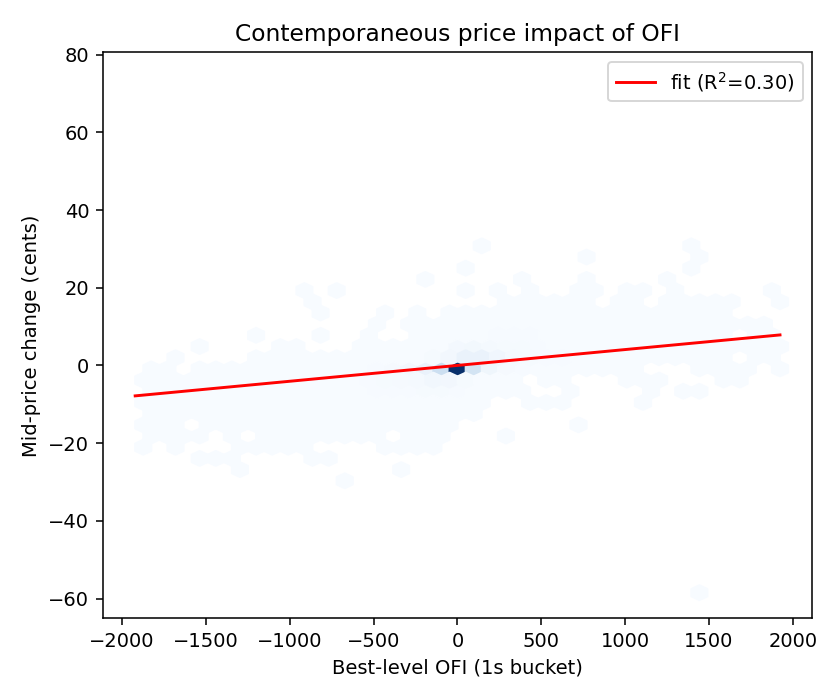
\includegraphics[width=0.52\textwidth]{outputs/fig1_impact.png}\hfill
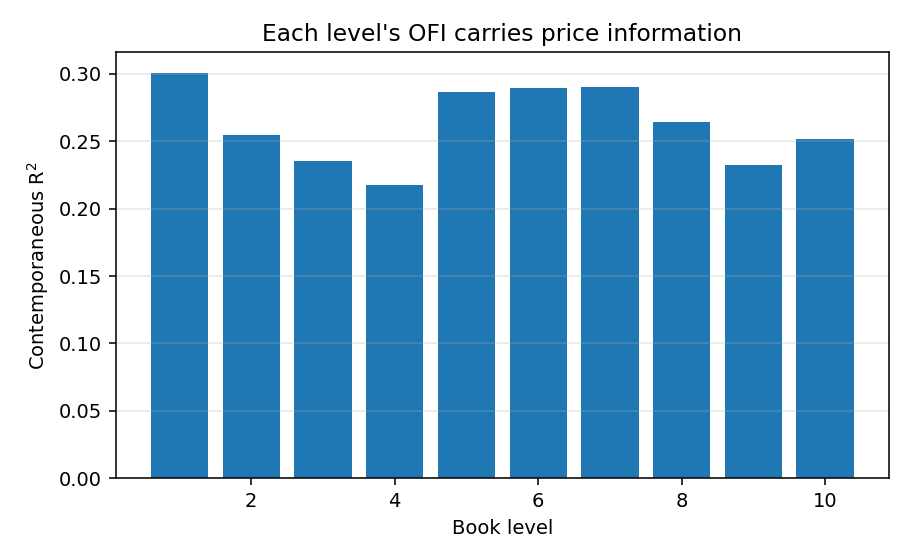
\includegraphics[width=0.46\textwidth]{outputs/fig2_level_r2.png}
\caption{Left: contemporaneous price impact --- mid-price change versus best-level
OFI (1s buckets), with the fitted line. Right: each book level's OFI explains
price change individually.}
\label{fig:impact}\label{fig:levels}
\end{figure}

\subsection{Robustness across time scales}
The relationship strengthens monotonically as the aggregation horizon lengthens
(Table~\ref{tab:scales}, Figure~\ref{fig:scales}): multi-level $R^2$ rises from
$0.51$ at one second to $0.74$ at thirty seconds. This is the expected effect of
averaging out event-level microstructure noise, and the ordering
best $<$ integrated $<$ multi-level is preserved at every scale.

\begin{table}[h]
\centering
\begin{tabular}{lcccc}
\toprule
Bucket & 1s & 5s & 10s & 30s \\
\midrule
Best-level & 0.301 & 0.369 & 0.411 & 0.480 \\
Integrated & 0.485 & 0.624 & 0.647 & 0.707 \\
Multi-level & 0.505 & 0.636 & 0.668 & 0.737 \\
\bottomrule
\end{tabular}
\caption{Contemporaneous $R^2$ across aggregation horizons.}
\label{tab:scales}
\end{table}

\begin{figure}[h]
\centering
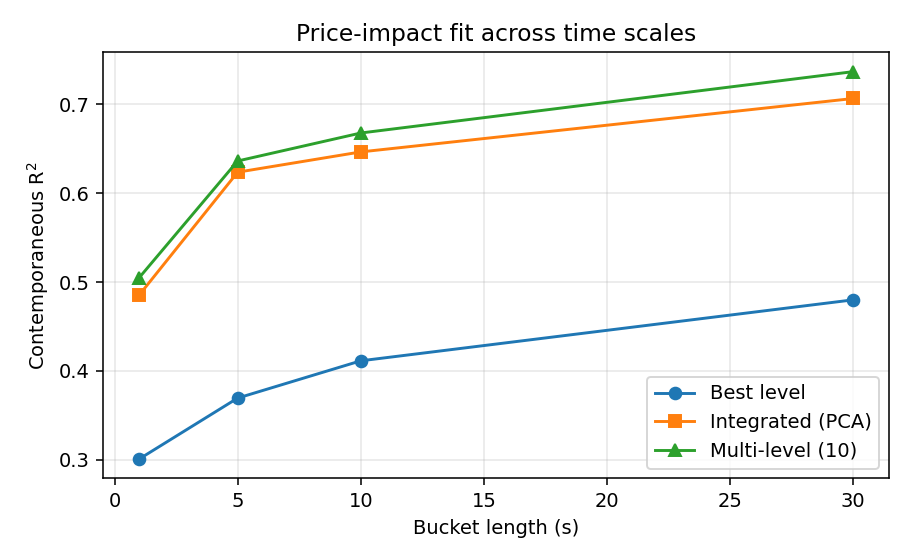
\includegraphics[width=0.52\textwidth]{outputs/fig3_scales.png}\hfill
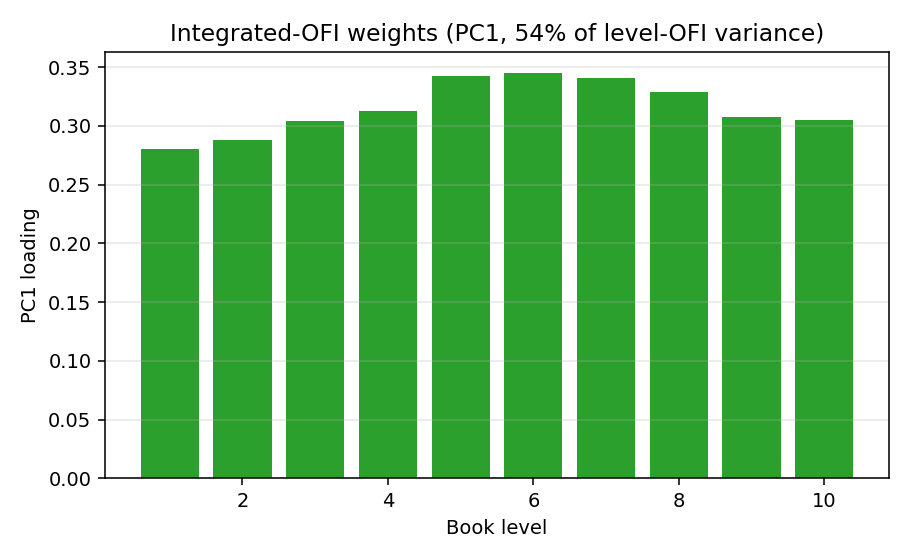
\includegraphics[width=0.46\textwidth]{outputs/fig4_pc1.png}
\caption{Left: explanatory power versus bucket length. Right: the integrated-OFI
weights (first principal component of the ten level OFIs).}
\label{fig:scales}
\end{figure}

\subsection{Prediction is a different question}
When the same OFI is used to forecast the \emph{next} bucket's return, out-of-sample
$R^2$ collapses to $0.0071$ for best-level OFI and $0.0070$ for the integrated
factor --- essentially zero. This is not a failure of the model; it is the correct
and expected result. OFI is contemporaneous with price formation: it measures the
pressure that is \emph{moving} the price now, not a signal that the market has left
un-arbitraged for the next second. The gap between a contemporaneous $R^2$ of
$0.5$ and a predictive $R^2$ of $0.007$ is precisely the gap between describing
microstructure and forecasting it, and honest evaluation must keep the two apart.

\section{Deepening the Analysis}
Four further analyses, all on the same real AAPL data, sharpen the picture.

\subsection{The impact of OFI is approximately linear}
Binning OFI into quantiles and plotting the mean mid-price change per bin
(Figure~\ref{fig:lin}) gives a strikingly straight relationship: a linear fit to
the binned curve attains $R^2 = 0.94$, higher than a fitted power law
($R^2 = 0.82$; log-log slope $0.35$, with mild concavity only at the extremes).
This linearity is a known and distinctive feature of \emph{order flow imbalance} ---
unlike the impact of raw traded volume, which is famously concave (square-root),
OFI enters price approximately linearly \cite{cks2014}. It is what makes OFI such a
convenient impact variable: a single coefficient $\lambda$ summarizes the response.

\subsection{The impact is permanent, not transient}
Regressing the cumulative mid-price change from the start of bucket $t$ to the end
of bucket $t+\ell$ on $\mathrm{OFI}_t$ gives an impact coefficient $\lambda(\ell)$
as a function of horizon (Figure~\ref{fig:decay}). It does not decay: starting at
$\lambda(0) = 4.1\times10^{-3}$ it is $5.3\times10^{-3}$ after twenty seconds ---
about $131\%$ of the immediate move. The price does not revert after an OFI shock;
if anything it continues to drift in the same direction. This is the signature of
\emph{information}, not transient liquidity pressure: order flow imbalance moves the
price and the move sticks, consistent with OFI reflecting genuine revisions in
valuation rather than temporary inventory effects.

\begin{figure}[h]
\centering
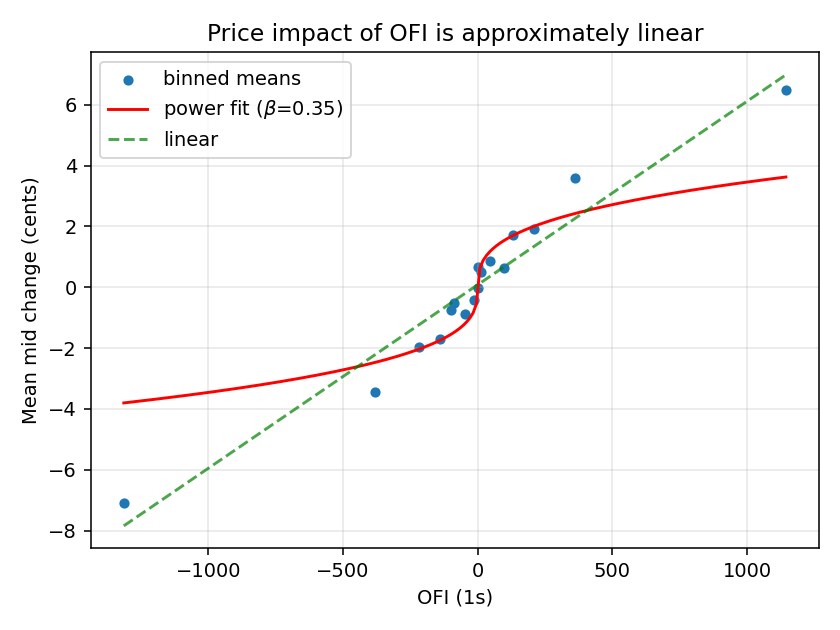
\includegraphics[width=0.49\textwidth]{outputs/fig5_linearity.png}\hfill
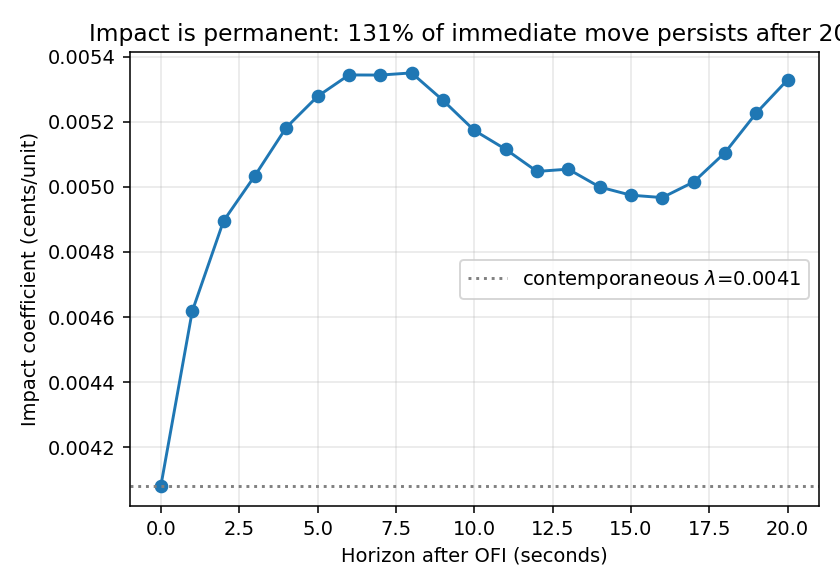
\includegraphics[width=0.49\textwidth]{outputs/fig6_decay.png}
\caption{Left: the binned impact curve is close to linear. Right: the impact
coefficient does not decay with horizon --- the price move is permanent.}
\label{fig:lin}\label{fig:decay}
\end{figure}

\subsection{The impact coefficient varies through the day}
Estimating $\lambda$ in thirty-minute bins (Figure~\ref{fig:intraday}) shows it is
not constant: it ranges from $2.6\times10^{-3}$ to $8.2\times10^{-3}$ cents per unit
across the session --- a roughly threefold variation, with the largest impact near
the open when depth is thin and each unit of imbalance moves price more. A fixed-$\lambda$
model is therefore a convenience, not a law; impact is state-dependent.

\subsection{Predictive power is negligible at every horizon}
Extending the out-of-sample predictive test to horizons of one, two, five, and ten
seconds (Figure~\ref{fig:predh}) confirms the earlier result at every horizon: the
held-out $R^2$ is $0.006$, $0.005$, $0.003$, and $0.002$ respectively --- small and
shrinking. Whatever information OFI carries is incorporated essentially
instantaneously; none of it survives as exploitable predictability a second or more
later.

\begin{figure}[h]
\centering
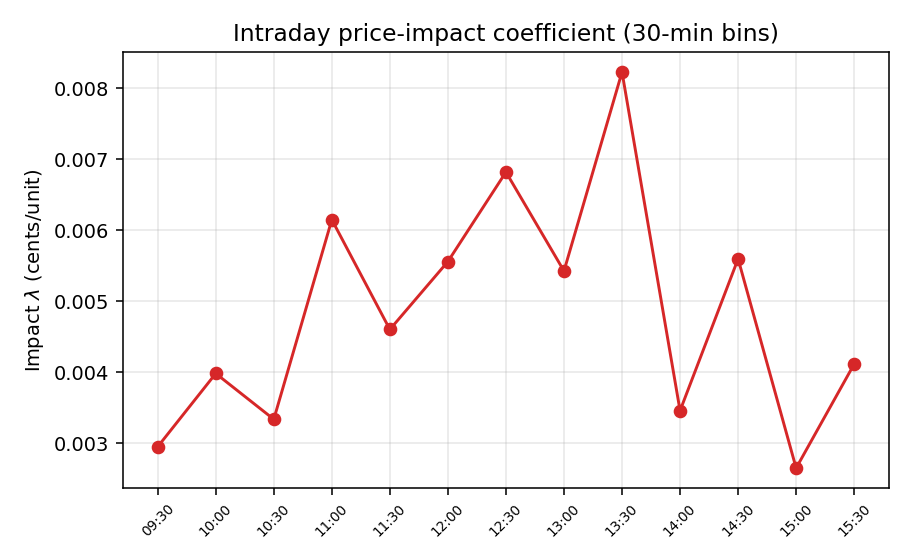
\includegraphics[width=0.49\textwidth]{outputs/fig7_intraday.png}\hfill
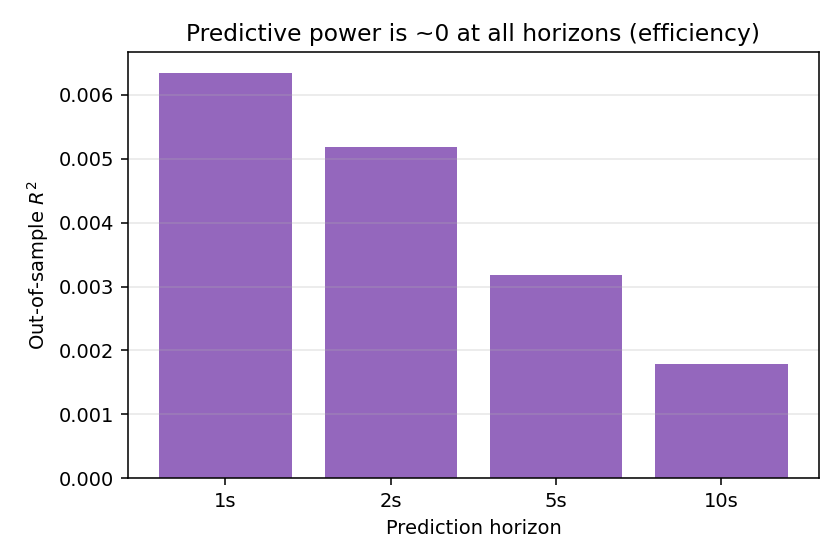
\includegraphics[width=0.49\textwidth]{outputs/fig8_pred_horizon.png}
\caption{Left: the price-impact coefficient varies about threefold intraday.
Right: out-of-sample predictive $R^2$ is negligible at all horizons.}
\label{fig:intraday}\label{fig:predh}
\end{figure}

\section{Discussion}
Two conclusions stand out. First, the \emph{depth of the book matters}: moving from
best-level to all ten levels lifts contemporaneous $R^2$ by about twenty points,
and a single integrated factor captures nearly all of that, so the extra signal is
real but low-dimensional. Second, \emph{contemporaneous is not predictive}: the
same variable that explains half of concurrent price variation forecasts almost
none of it out of sample. For execution and impact modelling --- sizing the price
move a given order flow will cause --- the contemporaneous relationship is exactly
what matters; for alpha, OFI at these horizons is close to efficient.

\paragraph{Limitations and extensions.} This is one asset on one day, so the
estimates are illustrative rather than universal; the clean way to generalize is to
repeat across names and dates. The most substantive extension is \emph{cross}-impact:
with synchronized multi-asset data, one estimates how asset $j$'s OFI moves asset
$i$'s price \cite{ccz2023}, and whether a cross-asset integrated factor improves on
per-asset OFI. That requires multi-ticker LOBSTER or vendor data and is the natural
next step. Other directions include a non-linear (concave) impact specification and
an intraday-varying $\lambda$.

\section{Reproducibility}
All numbers and figures come from a single script (included in
Appendix~A) that depends only on NumPy, pandas, and Matplotlib. The computation is
deterministic. The data is the public LOBSTER AAPL sample; it is not redistributed
with the code, which reads it from a local path (see the repository README for the
source).

\appendix
\section{Source Code: core analysis}
\lstinputlisting[style=py]{ofi_analysis.py}

\section{Source Code: extensions}
\lstinputlisting[style=py]{ofi_extensions.py}

\begin{thebibliography}{9}
\bibitem{cks2014} Cont, R., Kukanov, A., \& Stoikov, S. (2014). The price impact
of order book events. \textit{Journal of Financial Econometrics}, 12(1), 47--88.
\bibitem{ccz2023} Cont, R., Cucuringu, M., \& Zhang, C. (2023). Cross-impact of
order flow imbalance in equity markets. \textit{Quantitative Finance}, 23(10),
1373--1393.
\bibitem{lobster} Huang, R., \& Polak, T. LOBSTER: Limit Order Book System ---
the efficient reconstructor. Sample data, AAPL 2012-06-21.
\end{thebibliography}

\end{document}
